% Options for packages loaded elsewhere
\PassOptionsToPackage{unicode}{hyperref}
\PassOptionsToPackage{hyphens}{url}
\PassOptionsToPackage{dvipsnames,svgnames,x11names}{xcolor}
%
\documentclass[
  letterpaper,
  DIV=11,
  numbers=noendperiod]{scrartcl}

\usepackage{amsmath,amssymb}
\usepackage{iftex}
\ifPDFTeX
  \usepackage[T1]{fontenc}
  \usepackage[utf8]{inputenc}
  \usepackage{textcomp} % provide euro and other symbols
\else % if luatex or xetex
  \usepackage{unicode-math}
  \defaultfontfeatures{Scale=MatchLowercase}
  \defaultfontfeatures[\rmfamily]{Ligatures=TeX,Scale=1}
\fi
\usepackage{lmodern}
\ifPDFTeX\else  
    % xetex/luatex font selection
\fi
% Use upquote if available, for straight quotes in verbatim environments
\IfFileExists{upquote.sty}{\usepackage{upquote}}{}
\IfFileExists{microtype.sty}{% use microtype if available
  \usepackage[]{microtype}
  \UseMicrotypeSet[protrusion]{basicmath} % disable protrusion for tt fonts
}{}
\makeatletter
\@ifundefined{KOMAClassName}{% if non-KOMA class
  \IfFileExists{parskip.sty}{%
    \usepackage{parskip}
  }{% else
    \setlength{\parindent}{0pt}
    \setlength{\parskip}{6pt plus 2pt minus 1pt}}
}{% if KOMA class
  \KOMAoptions{parskip=half}}
\makeatother
\usepackage{xcolor}
\setlength{\emergencystretch}{3em} % prevent overfull lines
\setcounter{secnumdepth}{5}
% Make \paragraph and \subparagraph free-standing
\makeatletter
\ifx\paragraph\undefined\else
  \let\oldparagraph\paragraph
  \renewcommand{\paragraph}{
    \@ifstar
      \xxxParagraphStar
      \xxxParagraphNoStar
  }
  \newcommand{\xxxParagraphStar}[1]{\oldparagraph*{#1}\mbox{}}
  \newcommand{\xxxParagraphNoStar}[1]{\oldparagraph{#1}\mbox{}}
\fi
\ifx\subparagraph\undefined\else
  \let\oldsubparagraph\subparagraph
  \renewcommand{\subparagraph}{
    \@ifstar
      \xxxSubParagraphStar
      \xxxSubParagraphNoStar
  }
  \newcommand{\xxxSubParagraphStar}[1]{\oldsubparagraph*{#1}\mbox{}}
  \newcommand{\xxxSubParagraphNoStar}[1]{\oldsubparagraph{#1}\mbox{}}
\fi
\makeatother

\usepackage{color}
\usepackage{fancyvrb}
\newcommand{\VerbBar}{|}
\newcommand{\VERB}{\Verb[commandchars=\\\{\}]}
\DefineVerbatimEnvironment{Highlighting}{Verbatim}{commandchars=\\\{\}}
% Add ',fontsize=\small' for more characters per line
\newenvironment{Shaded}{}{}
\newcommand{\AlertTok}[1]{\textcolor[rgb]{1.00,0.33,0.33}{\textbf{#1}}}
\newcommand{\AnnotationTok}[1]{\textcolor[rgb]{0.42,0.45,0.49}{#1}}
\newcommand{\AttributeTok}[1]{\textcolor[rgb]{0.84,0.23,0.29}{#1}}
\newcommand{\BaseNTok}[1]{\textcolor[rgb]{0.00,0.36,0.77}{#1}}
\newcommand{\BuiltInTok}[1]{\textcolor[rgb]{0.84,0.23,0.29}{#1}}
\newcommand{\CharTok}[1]{\textcolor[rgb]{0.01,0.18,0.38}{#1}}
\newcommand{\CommentTok}[1]{\textcolor[rgb]{0.42,0.45,0.49}{#1}}
\newcommand{\CommentVarTok}[1]{\textcolor[rgb]{0.42,0.45,0.49}{#1}}
\newcommand{\ConstantTok}[1]{\textcolor[rgb]{0.00,0.36,0.77}{#1}}
\newcommand{\ControlFlowTok}[1]{\textcolor[rgb]{0.84,0.23,0.29}{#1}}
\newcommand{\DataTypeTok}[1]{\textcolor[rgb]{0.84,0.23,0.29}{#1}}
\newcommand{\DecValTok}[1]{\textcolor[rgb]{0.00,0.36,0.77}{#1}}
\newcommand{\DocumentationTok}[1]{\textcolor[rgb]{0.42,0.45,0.49}{#1}}
\newcommand{\ErrorTok}[1]{\textcolor[rgb]{1.00,0.33,0.33}{\underline{#1}}}
\newcommand{\ExtensionTok}[1]{\textcolor[rgb]{0.84,0.23,0.29}{\textbf{#1}}}
\newcommand{\FloatTok}[1]{\textcolor[rgb]{0.00,0.36,0.77}{#1}}
\newcommand{\FunctionTok}[1]{\textcolor[rgb]{0.44,0.26,0.76}{#1}}
\newcommand{\ImportTok}[1]{\textcolor[rgb]{0.01,0.18,0.38}{#1}}
\newcommand{\InformationTok}[1]{\textcolor[rgb]{0.42,0.45,0.49}{#1}}
\newcommand{\KeywordTok}[1]{\textcolor[rgb]{0.84,0.23,0.29}{#1}}
\newcommand{\NormalTok}[1]{\textcolor[rgb]{0.14,0.16,0.18}{#1}}
\newcommand{\OperatorTok}[1]{\textcolor[rgb]{0.14,0.16,0.18}{#1}}
\newcommand{\OtherTok}[1]{\textcolor[rgb]{0.44,0.26,0.76}{#1}}
\newcommand{\PreprocessorTok}[1]{\textcolor[rgb]{0.84,0.23,0.29}{#1}}
\newcommand{\RegionMarkerTok}[1]{\textcolor[rgb]{0.42,0.45,0.49}{#1}}
\newcommand{\SpecialCharTok}[1]{\textcolor[rgb]{0.00,0.36,0.77}{#1}}
\newcommand{\SpecialStringTok}[1]{\textcolor[rgb]{0.01,0.18,0.38}{#1}}
\newcommand{\StringTok}[1]{\textcolor[rgb]{0.01,0.18,0.38}{#1}}
\newcommand{\VariableTok}[1]{\textcolor[rgb]{0.89,0.38,0.04}{#1}}
\newcommand{\VerbatimStringTok}[1]{\textcolor[rgb]{0.01,0.18,0.38}{#1}}
\newcommand{\WarningTok}[1]{\textcolor[rgb]{1.00,0.33,0.33}{#1}}

\providecommand{\tightlist}{%
  \setlength{\itemsep}{0pt}\setlength{\parskip}{0pt}}\usepackage{longtable,booktabs,array}
\usepackage{calc} % for calculating minipage widths
% Correct order of tables after \paragraph or \subparagraph
\usepackage{etoolbox}
\makeatletter
\patchcmd\longtable{\par}{\if@noskipsec\mbox{}\fi\par}{}{}
\makeatother
% Allow footnotes in longtable head/foot
\IfFileExists{footnotehyper.sty}{\usepackage{footnotehyper}}{\usepackage{footnote}}
\makesavenoteenv{longtable}
\usepackage{graphicx}
\makeatletter
\newsavebox\pandoc@box
\newcommand*\pandocbounded[1]{% scales image to fit in text height/width
  \sbox\pandoc@box{#1}%
  \Gscale@div\@tempa{\textheight}{\dimexpr\ht\pandoc@box+\dp\pandoc@box\relax}%
  \Gscale@div\@tempb{\linewidth}{\wd\pandoc@box}%
  \ifdim\@tempb\p@<\@tempa\p@\let\@tempa\@tempb\fi% select the smaller of both
  \ifdim\@tempa\p@<\p@\scalebox{\@tempa}{\usebox\pandoc@box}%
  \else\usebox{\pandoc@box}%
  \fi%
}
% Set default figure placement to htbp
\def\fps@figure{htbp}
\makeatother

\usepackage{booktabs}
\usepackage{longtable}
\usepackage{array}
\usepackage{multirow}
\usepackage{wrapfig}
\usepackage{float}
\usepackage{colortbl}
\usepackage{pdflscape}
\usepackage{tabu}
\usepackage{threeparttable}
\usepackage{threeparttablex}
\usepackage[normalem]{ulem}
\usepackage{makecell}
\usepackage{xcolor}
\KOMAoption{captions}{tableheading}
\makeatletter
\@ifpackageloaded{caption}{}{\usepackage{caption}}
\AtBeginDocument{%
\ifdefined\contentsname
  \renewcommand*\contentsname{Table of contents}
\else
  \newcommand\contentsname{Table of contents}
\fi
\ifdefined\listfigurename
  \renewcommand*\listfigurename{List of Figures}
\else
  \newcommand\listfigurename{List of Figures}
\fi
\ifdefined\listtablename
  \renewcommand*\listtablename{List of Tables}
\else
  \newcommand\listtablename{List of Tables}
\fi
\ifdefined\figurename
  \renewcommand*\figurename{Figure}
\else
  \newcommand\figurename{Figure}
\fi
\ifdefined\tablename
  \renewcommand*\tablename{Table}
\else
  \newcommand\tablename{Table}
\fi
}
\@ifpackageloaded{float}{}{\usepackage{float}}
\floatstyle{ruled}
\@ifundefined{c@chapter}{\newfloat{codelisting}{h}{lop}}{\newfloat{codelisting}{h}{lop}[chapter]}
\floatname{codelisting}{Listing}
\newcommand*\listoflistings{\listof{codelisting}{List of Listings}}
\makeatother
\makeatletter
\makeatother
\makeatletter
\@ifpackageloaded{caption}{}{\usepackage{caption}}
\@ifpackageloaded{subcaption}{}{\usepackage{subcaption}}
\makeatother

\usepackage{bookmark}

\IfFileExists{xurl.sty}{\usepackage{xurl}}{} % add URL line breaks if available
\urlstyle{same} % disable monospaced font for URLs
\hypersetup{
  pdftitle={Supplementary Materials of Impact of IPTp Regimen on Pregnancy Outcomes},
  colorlinks=true,
  linkcolor={blue},
  filecolor={Maroon},
  citecolor={Blue},
  urlcolor={Blue},
  pdfcreator={LaTeX via pandoc}}


\title{Supplementary Materials of Impact of IPTp Regimen on Pregnancy
Outcomes}
\author{}
\date{}

\begin{document}
\maketitle


\newpage{}

\section{Overview}\label{overview}

The Supplementary Appendix begins with comprehensive methodological
details, including variable‐by‐variable missingness (Table S1), analysis
of deviance comparing models with and without the malaria×SP interaction
(Table S2), and variance inflation factors for the final interaction
model (Table S3). It also presents machine‐learning tuning results with
the top five elastic-net hyperparameter combinations ranked by mean
cross-validated AUC (Table S4) alongside a heatmap illustrating AUC
across the penalty--mixture grid (Figure S1). Full code excerpts
document our data-cleaning steps, rsample splits, recipe definitions,
and tune\_grid workflows. The appendix then moves on to additional
results: a detailed stratification of outcome measures and
malaria-exposure variables by IPTp arm (Table S5), bar graphs of total
malaria episodes during pregnancy (Figure S2), gravidity (Figure S3),
and parity (Figure S4) distributions by treatment arm, and a bootstrap
calibration curve for the interaction model (Figure S5). Finally, it
compares model discrimination with overlaid ROC curves for logistic
regression, random forest, and XGBoost (Figure S6), presents a
precision-recall curve for the top‐performing machine-learning model
(Figure S7), and reports the test-set AUC for the gravidity-only model
in women under 25 years (Table S6).

\section{Code and file information}\label{code-and-file-information}

Explain here what each code/file is and does, and in which order (if
any) users need to run thing to reproduce everything. Essentially, give
a full set of instructions to re-generate everything.

\newpage{}

\section{Additional Method Details}\label{additional-method-details}

Often, the main manuscript only allows for an overview description of
the methods. Use the supplement to describe all your methods, models and
approaches in a lot of detail. Reference specific parts of your code as
needed.

\newpage{}

\section{Additional results}\label{additional-results}

Show additional results here. Those can be some useful
exploratory/descriptive figures or tables, or results from additional
analyses that didn't make it into the main text.

\emph{Bar Graph of Total Malaria Episodes During Pregnancy by Treatment
Arm}

\begin{Shaded}
\begin{Highlighting}[]
\CommentTok{\# Load necessary libraries}
\FunctionTok{library}\NormalTok{(dplyr)}
\FunctionTok{library}\NormalTok{(ggplot2)}
\FunctionTok{library}\NormalTok{(here)}

\CommentTok{\# Read in the cleaned data}
\NormalTok{promo\_data\_clean }\OtherTok{\textless{}{-}} \FunctionTok{read.csv}\NormalTok{(}\FunctionTok{here}\NormalTok{(}\StringTok{"data"}\NormalTok{, }\StringTok{"clean"}\NormalTok{, }\StringTok{"PROMO\_Data\_clean.csv"}\NormalTok{))}

\CommentTok{\# Recode \textquotesingle{}total\_malaria\_episodes\_during\_pregnancy\textquotesingle{} into a categorical variable}
\NormalTok{promo\_data\_clean }\OtherTok{\textless{}{-}}\NormalTok{ promo\_data\_clean }\SpecialCharTok{\%\textgreater{}\%}
  \FunctionTok{mutate}\NormalTok{(}
    \AttributeTok{MalariaEpisodesPreg\_cat =} \FunctionTok{case\_when}\NormalTok{(}
\NormalTok{      total\_malaria\_episodes\_during\_pregnancy }\SpecialCharTok{\%in\%} \FunctionTok{c}\NormalTok{(}\DecValTok{0}\NormalTok{, }\DecValTok{1}\NormalTok{) }\SpecialCharTok{\textasciitilde{}} \StringTok{"1"}\NormalTok{,}
\NormalTok{      total\_malaria\_episodes\_during\_pregnancy }\SpecialCharTok{\%in\%} \FunctionTok{c}\NormalTok{(}\DecValTok{2}\NormalTok{, }\DecValTok{3}\NormalTok{) }\SpecialCharTok{\textasciitilde{}} \StringTok{"2–3"}\NormalTok{,}
\NormalTok{      total\_malaria\_episodes\_during\_pregnancy }\SpecialCharTok{\textgreater{}=} \DecValTok{4} \SpecialCharTok{\textasciitilde{}} \StringTok{"≥4"}
\NormalTok{    ),}
    \AttributeTok{MalariaEpisodesPreg\_cat =} \FunctionTok{factor}\NormalTok{(MalariaEpisodesPreg\_cat, }\AttributeTok{levels =} \FunctionTok{c}\NormalTok{(}\StringTok{"1"}\NormalTok{, }\StringTok{"2–3"}\NormalTok{, }\StringTok{"≥4"}\NormalTok{))}
\NormalTok{  )}

\CommentTok{\# Create the bar graph}
\FunctionTok{ggplot}\NormalTok{(promo\_data\_clean, }\FunctionTok{aes}\NormalTok{(}\AttributeTok{x =}\NormalTok{ MalariaEpisodesPreg\_cat, }\AttributeTok{fill =}\NormalTok{ study\_arm)) }\SpecialCharTok{+}
  \FunctionTok{geom\_bar}\NormalTok{(}\AttributeTok{position =} \StringTok{"dodge"}\NormalTok{) }\SpecialCharTok{+}
  \FunctionTok{labs}\NormalTok{(}\AttributeTok{title =} \StringTok{"Total Malaria Episodes During Pregnancy by Treatment Arm"}\NormalTok{,}
       \AttributeTok{x =} \StringTok{"Total Malaria Episodes During Pregnancy (Categorical)"}\NormalTok{,}
       \AttributeTok{y =} \StringTok{"Count"}\NormalTok{,}
       \AttributeTok{fill =} \StringTok{"Treatment Arm"}\NormalTok{) }\SpecialCharTok{+}
  \FunctionTok{theme\_minimal}\NormalTok{()}
\end{Highlighting}
\end{Shaded}

\pandocbounded{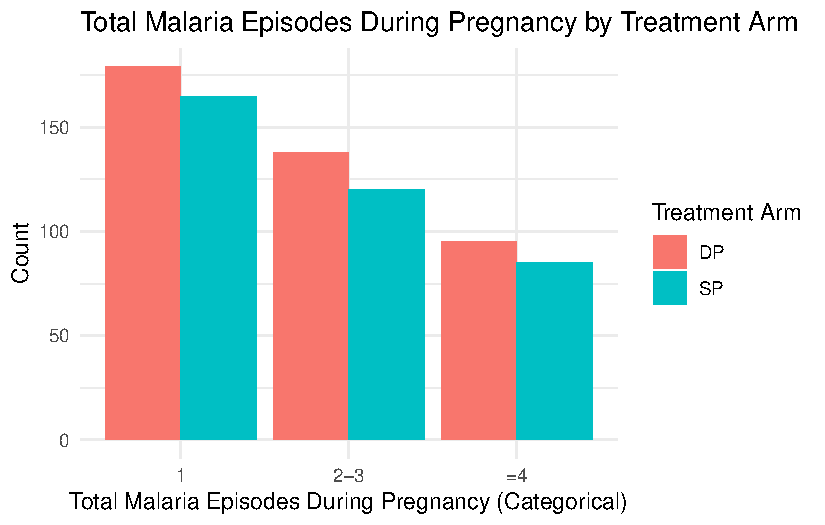
\includegraphics[keepaspectratio]{Supplementary-Material_files/figure-pdf/unnamed-chunk-4-1.pdf}}

\emph{Bar Graphs for Gravidity and Parity}

\begin{Shaded}
\begin{Highlighting}[]
\CommentTok{\# Load necessary libraries}

\CommentTok{\# Read in the cleaned data}
\NormalTok{promo\_data\_clean }\OtherTok{\textless{}{-}} \FunctionTok{read.csv}\NormalTok{(}\FunctionTok{here}\NormalTok{(}\StringTok{"data"}\NormalTok{, }\StringTok{"clean"}\NormalTok{, }\StringTok{"PROMO\_Data\_clean.csv"}\NormalTok{))}

\CommentTok{\# Recode Gravidity into categories: "1", "2–3", "≥4"}
\NormalTok{promo\_data\_clean }\OtherTok{\textless{}{-}}\NormalTok{ promo\_data\_clean }\SpecialCharTok{\%\textgreater{}\%}
  \FunctionTok{mutate}\NormalTok{(}
    \AttributeTok{Gravidity\_cat =} \FunctionTok{case\_when}\NormalTok{(}
\NormalTok{      gravidity }\SpecialCharTok{==} \DecValTok{1} \SpecialCharTok{\textasciitilde{}} \StringTok{"1"}\NormalTok{,}
\NormalTok{      gravidity }\SpecialCharTok{\%in\%} \FunctionTok{c}\NormalTok{(}\DecValTok{2}\NormalTok{, }\DecValTok{3}\NormalTok{) }\SpecialCharTok{\textasciitilde{}} \StringTok{"2–3"}\NormalTok{,}
\NormalTok{      gravidity }\SpecialCharTok{\textgreater{}=} \DecValTok{4} \SpecialCharTok{\textasciitilde{}} \StringTok{"≥4"}
\NormalTok{    ),}
    \AttributeTok{Gravidity\_cat =} \FunctionTok{factor}\NormalTok{(Gravidity\_cat, }\AttributeTok{levels =} \FunctionTok{c}\NormalTok{(}\StringTok{"1"}\NormalTok{, }\StringTok{"2–3"}\NormalTok{, }\StringTok{"≥4"}\NormalTok{))}
\NormalTok{  )}

\CommentTok{\# Create the bar graph for Gravidity by Treatment Arm}
\FunctionTok{ggplot}\NormalTok{(promo\_data\_clean, }\FunctionTok{aes}\NormalTok{(}\AttributeTok{x =}\NormalTok{ Gravidity\_cat, }\AttributeTok{fill =}\NormalTok{ study\_arm)) }\SpecialCharTok{+}
  \FunctionTok{geom\_bar}\NormalTok{(}\AttributeTok{position =} \StringTok{"dodge"}\NormalTok{) }\SpecialCharTok{+}
  \FunctionTok{labs}\NormalTok{(}\AttributeTok{title =} \StringTok{"Gravidity Distribution by Treatment Arm"}\NormalTok{,}
       \AttributeTok{x =} \StringTok{"Gravidity Category (1, 2–3, ≥4)"}\NormalTok{,}
       \AttributeTok{y =} \StringTok{"Count"}\NormalTok{,}
       \AttributeTok{fill =} \StringTok{"Treatment Arm"}\NormalTok{) }\SpecialCharTok{+}
  \FunctionTok{theme\_minimal}\NormalTok{()}
\end{Highlighting}
\end{Shaded}

\pandocbounded{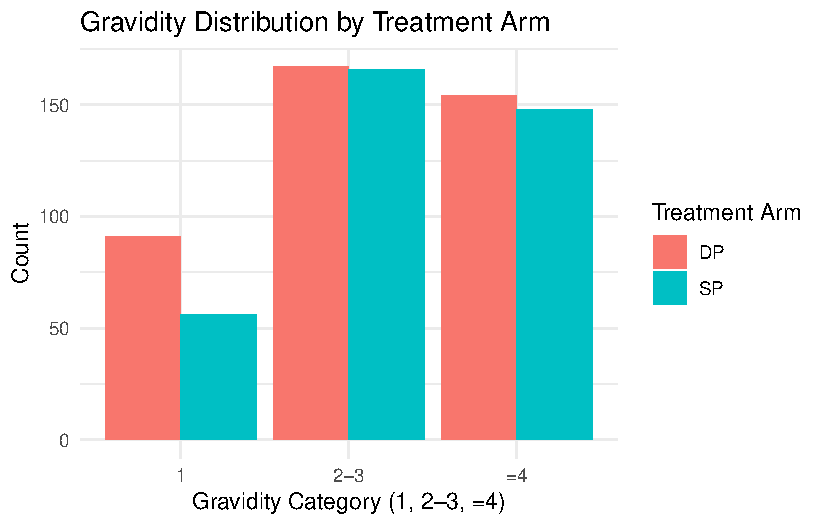
\includegraphics[keepaspectratio]{Supplementary-Material_files/figure-pdf/unnamed-chunk-5-1.pdf}}

\emph{Parity Distribution by Treatment Arm}

\begin{Shaded}
\begin{Highlighting}[]
\CommentTok{\# Load necessary libraries}
\FunctionTok{library}\NormalTok{(dplyr)}
\FunctionTok{library}\NormalTok{(ggplot2)}
\FunctionTok{library}\NormalTok{(here)}

\CommentTok{\# Read in the cleaned data}
\NormalTok{promo\_data\_clean }\OtherTok{\textless{}{-}} \FunctionTok{read.csv}\NormalTok{(}\FunctionTok{here}\NormalTok{(}\StringTok{"data"}\NormalTok{, }\StringTok{"clean"}\NormalTok{, }\StringTok{"PROMO\_Data\_clean.csv"}\NormalTok{))}

\CommentTok{\# Recode Parity into categories: "0", "1–2", "≥3"}
\NormalTok{promo\_data\_clean }\OtherTok{\textless{}{-}}\NormalTok{ promo\_data\_clean }\SpecialCharTok{\%\textgreater{}\%}
  \FunctionTok{mutate}\NormalTok{(}
    \AttributeTok{Parity\_cat =} \FunctionTok{case\_when}\NormalTok{(}
\NormalTok{      parity }\SpecialCharTok{==} \DecValTok{0} \SpecialCharTok{\textasciitilde{}} \StringTok{"0"}\NormalTok{,}
\NormalTok{      parity }\SpecialCharTok{\%in\%} \FunctionTok{c}\NormalTok{(}\DecValTok{1}\NormalTok{, }\DecValTok{2}\NormalTok{) }\SpecialCharTok{\textasciitilde{}} \StringTok{"1–2"}\NormalTok{,}
\NormalTok{      parity }\SpecialCharTok{\textgreater{}=} \DecValTok{3} \SpecialCharTok{\textasciitilde{}} \StringTok{"≥3"}
\NormalTok{    ),}
    \AttributeTok{Parity\_cat =} \FunctionTok{factor}\NormalTok{(Parity\_cat, }\AttributeTok{levels =} \FunctionTok{c}\NormalTok{(}\StringTok{"0"}\NormalTok{, }\StringTok{"1–2"}\NormalTok{, }\StringTok{"≥3"}\NormalTok{))}
\NormalTok{  )}

\CommentTok{\# Create the bar graph for Parity by Treatment Arm}
\FunctionTok{ggplot}\NormalTok{(promo\_data\_clean, }\FunctionTok{aes}\NormalTok{(}\AttributeTok{x =}\NormalTok{ Parity\_cat, }\AttributeTok{fill =}\NormalTok{ study\_arm)) }\SpecialCharTok{+}
  \FunctionTok{geom\_bar}\NormalTok{(}\AttributeTok{position =} \StringTok{"dodge"}\NormalTok{) }\SpecialCharTok{+}
  \FunctionTok{labs}\NormalTok{(}\AttributeTok{title =} \StringTok{"Parity Distribution by Treatment Arm"}\NormalTok{,}
       \AttributeTok{x =} \StringTok{"Parity Category (0, 1–2, ≥3)"}\NormalTok{,}
       \AttributeTok{y =} \StringTok{"Count"}\NormalTok{,}
       \AttributeTok{fill =} \StringTok{"Treatment Arm"}\NormalTok{) }\SpecialCharTok{+}
  \FunctionTok{theme\_minimal}\NormalTok{()}
\end{Highlighting}
\end{Shaded}

\pandocbounded{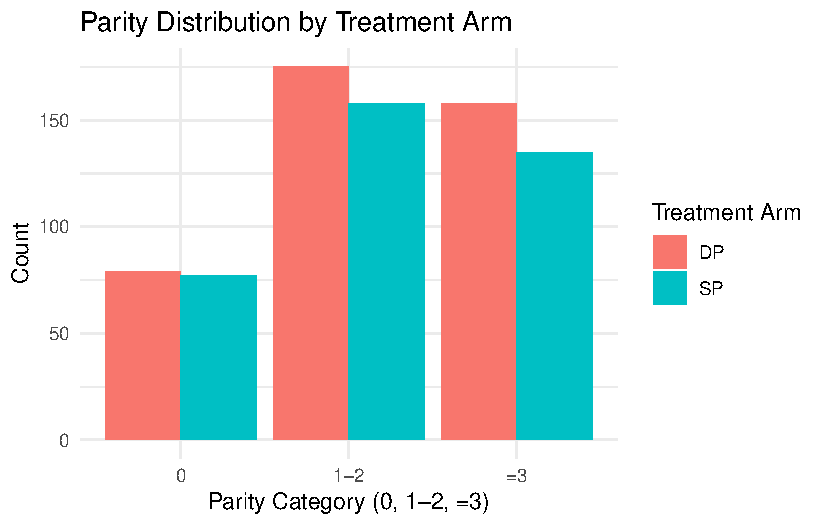
\includegraphics[keepaspectratio]{Supplementary-Material_files/figure-pdf/unnamed-chunk-6-1.pdf}}

\subsection{Example additional result}\label{example-additional-result}

Table~\ref{tbl-resulttable1} shows an additional table summarizing a
model fit.

\begin{longtable}[]{@{}lrrrr@{}}

\caption{\label{tbl-resulttable1}Another fit table.}

\tabularnewline

\toprule\noalign{}
term & estimate & std.error & statistic & p.value \\
\midrule\noalign{}
\endhead
\bottomrule\noalign{}
\endlastfoot
(Intercept) & 149.6997661 & 19.7518528 & 7.5790240 & 0.0001285 \\
Weight & 0.2277371 & 0.2708841 & 0.8407177 & 0.4282860 \\

\end{longtable}

Figure~\ref{fig-result2} shows a scatterplot figure produced by one of
the R scripts.

\begin{figure}

\centering{

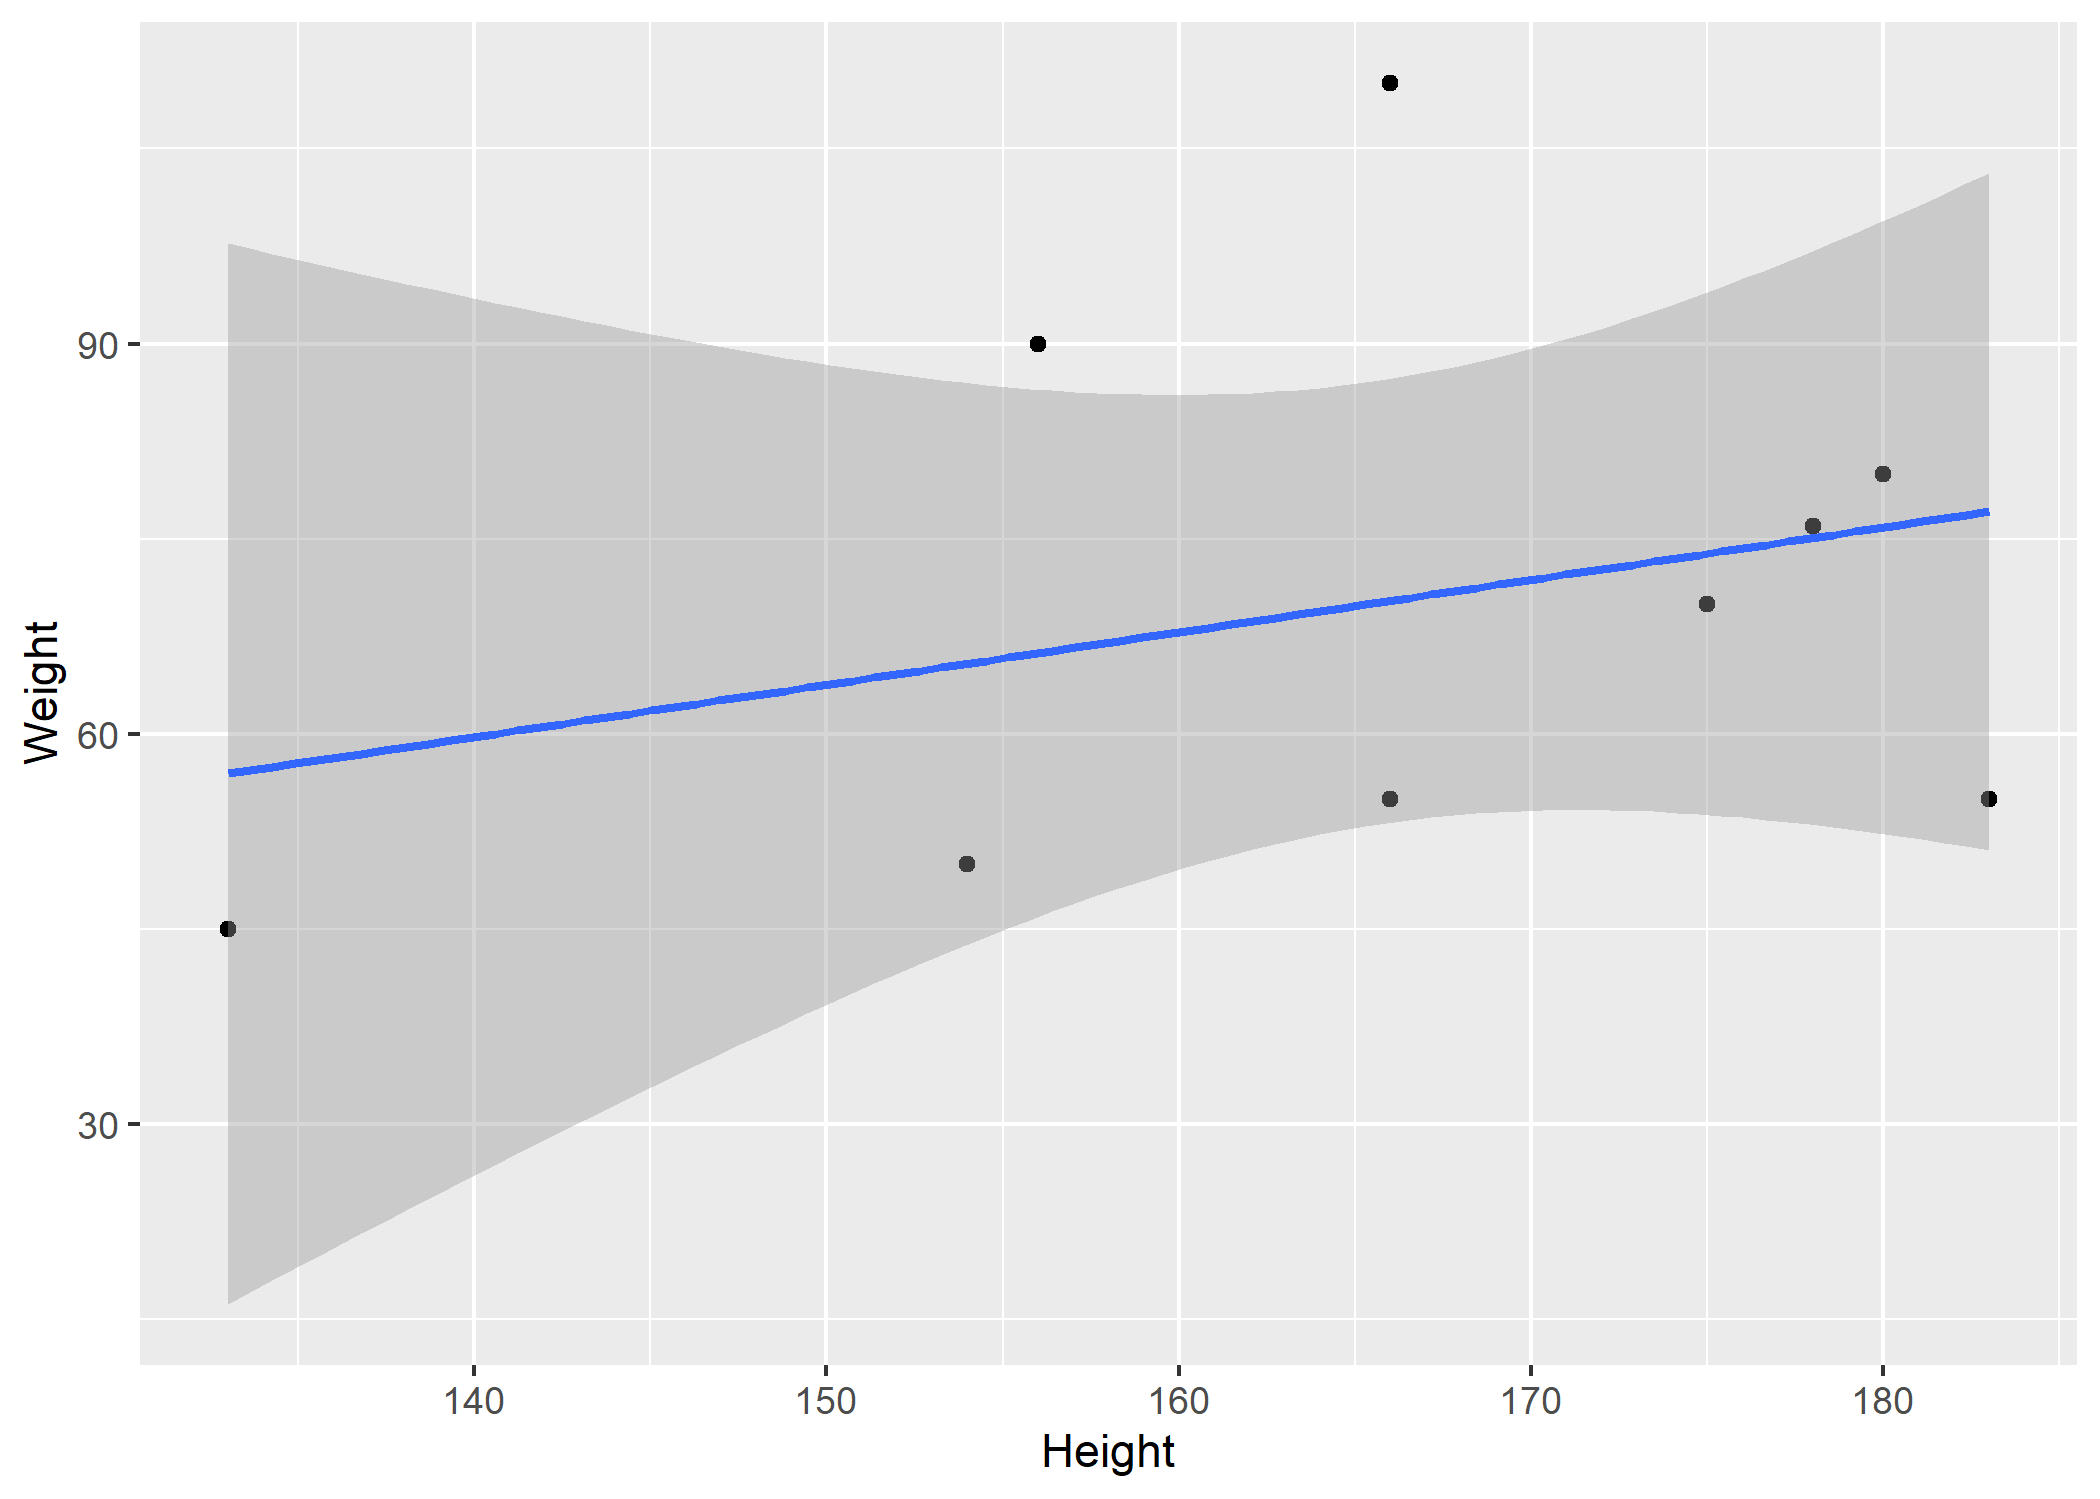
\includegraphics[width=7in,height=\textheight,keepaspectratio]{../../../results/figures/height-weight.png}

}

\caption{\label{fig-result2}Height and weight.}

\end{figure}%

\section{Evaluating Discrimination (ROC Curve and
AUC)}\label{evaluating-discrimination-roc-curve-and-auc}

\begin{Shaded}
\begin{Highlighting}[]
\CommentTok{\# 1) Load required libraries}
\FunctionTok{library}\NormalTok{(dplyr)}
\FunctionTok{library}\NormalTok{(pROC)}
\FunctionTok{library}\NormalTok{(caret)}
\FunctionTok{library}\NormalTok{(here)}

\CommentTok{\# 2) Read cleaned data and subset to women \textless{} 25}
\NormalTok{promo\_data\_clean }\OtherTok{\textless{}{-}} \FunctionTok{read.csv}\NormalTok{(}\FunctionTok{here}\NormalTok{(}\StringTok{"data/clean/PROMO\_Data\_clean.csv"}\NormalTok{))}
\NormalTok{promo\_data\_young }\OtherTok{\textless{}{-}}\NormalTok{ promo\_data\_clean }\SpecialCharTok{\%\textgreater{}\%}
  \FunctionTok{filter}\NormalTok{(age\_at\_enrollment\_years }\SpecialCharTok{\textless{}} \DecValTok{25}\NormalTok{) }\SpecialCharTok{\%\textgreater{}\%}
  \FunctionTok{mutate}\NormalTok{(}
    \CommentTok{\# Composite adverse outcome: 1 if preterm, stillbirth, or low birth weight}
    \AttributeTok{low\_birth\_weight      =} \FunctionTok{as.integer}\NormalTok{(birth\_weight }\SpecialCharTok{\textless{}} \FloatTok{2.5}\NormalTok{),}
    \AttributeTok{adverse\_birth\_outcome =} \FunctionTok{as.integer}\NormalTok{(}
\NormalTok{      preterm\_births\_count }\SpecialCharTok{\textgreater{}} \DecValTok{0} \SpecialCharTok{|}
\NormalTok{      stillbirth\_bin }\SpecialCharTok{==} \DecValTok{1}        \SpecialCharTok{|}
\NormalTok{      low\_birth\_weight }\SpecialCharTok{==} \DecValTok{1}
\NormalTok{    )}
\NormalTok{  )}

\CommentTok{\# 3) Fit logistic regression model}
\NormalTok{model\_gravidity }\OtherTok{\textless{}{-}} \FunctionTok{glm}\NormalTok{(}
\NormalTok{  adverse\_birth\_outcome }\SpecialCharTok{\textasciitilde{}}\NormalTok{ gravidity }\SpecialCharTok{+}\NormalTok{ total\_malaria\_episodes }\SpecialCharTok{+}
\NormalTok{    study\_arm }\SpecialCharTok{+}\NormalTok{ education\_level,}
  \AttributeTok{family =} \FunctionTok{binomial}\NormalTok{(}\AttributeTok{link =} \StringTok{"logit"}\NormalTok{),}
  \AttributeTok{data   =}\NormalTok{ promo\_data\_young}
\NormalTok{)}

\CommentTok{\# 4) Generate predicted probabilities}
\NormalTok{promo\_data\_young}\SpecialCharTok{$}\NormalTok{predicted\_prob }\OtherTok{\textless{}{-}} \FunctionTok{predict}\NormalTok{(}
\NormalTok{  model\_gravidity,}
  \AttributeTok{newdata =}\NormalTok{ promo\_data\_young,}
  \AttributeTok{type    =} \StringTok{"response"}
\NormalTok{)}

\CommentTok{\# 5) ROC curve and AUC}
\NormalTok{roc\_obj  }\OtherTok{\textless{}{-}} \FunctionTok{roc}\NormalTok{(}
\NormalTok{  promo\_data\_young}\SpecialCharTok{$}\NormalTok{adverse\_birth\_outcome,}
\NormalTok{  promo\_data\_young}\SpecialCharTok{$}\NormalTok{predicted\_prob}
\NormalTok{)}
\FunctionTok{plot}\NormalTok{(}
\NormalTok{  roc\_obj,}
  \AttributeTok{col   =} \StringTok{"blue"}\NormalTok{,}
  \AttributeTok{lwd   =} \DecValTok{2}\NormalTok{,}
  \AttributeTok{main  =} \StringTok{"ROC Curve: Gravidity Model (Age \textless{} 25)"}
\NormalTok{)}
\end{Highlighting}
\end{Shaded}

\pandocbounded{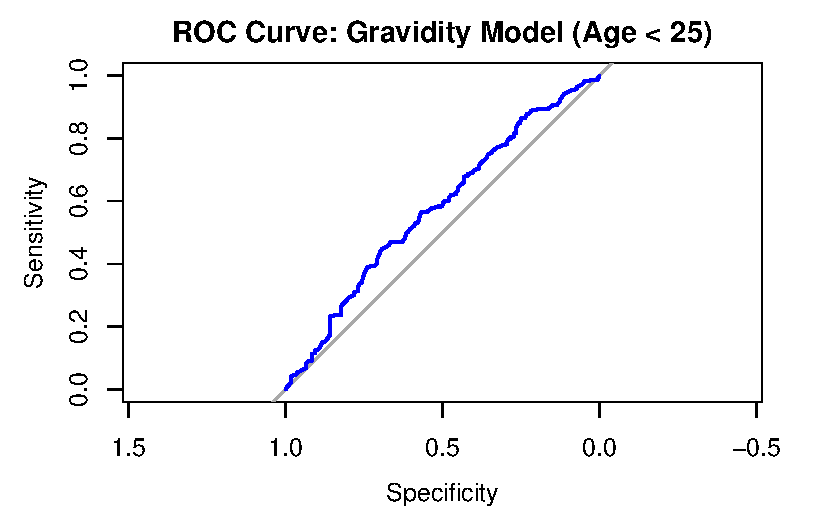
\includegraphics[keepaspectratio]{Supplementary-Material_files/figure-pdf/roc-calibration-1.pdf}}

\begin{Shaded}
\begin{Highlighting}[]
\NormalTok{auc\_val }\OtherTok{\textless{}{-}} \FunctionTok{auc}\NormalTok{(roc\_obj)}
\FunctionTok{cat}\NormalTok{(}\StringTok{"AUC:"}\NormalTok{, }\FunctionTok{round}\NormalTok{(auc\_val, }\DecValTok{2}\NormalTok{), }\StringTok{"}\SpecialCharTok{\textbackslash{}n}\StringTok{"}\NormalTok{)}
\end{Highlighting}
\end{Shaded}

\begin{verbatim}
AUC: 0.58 
\end{verbatim}

\begin{Shaded}
\begin{Highlighting}[]
\CommentTok{\# 6) Calibration plot}
\NormalTok{data\_cal }\OtherTok{\textless{}{-}} \FunctionTok{data.frame}\NormalTok{(}
  \AttributeTok{observed =} \FunctionTok{factor}\NormalTok{(promo\_data\_young}\SpecialCharTok{$}\NormalTok{adverse\_birth\_outcome, }\AttributeTok{levels =} \FunctionTok{c}\NormalTok{(}\DecValTok{0}\NormalTok{,}\DecValTok{1}\NormalTok{)),}
  \AttributeTok{predicted =}\NormalTok{ promo\_data\_young}\SpecialCharTok{$}\NormalTok{predicted\_prob}
\NormalTok{)}
\NormalTok{cal\_plot }\OtherTok{\textless{}{-}} \FunctionTok{calibration}\NormalTok{(}
\NormalTok{  observed }\SpecialCharTok{\textasciitilde{}}\NormalTok{ predicted,}
  \AttributeTok{data  =}\NormalTok{ data\_cal,}
  \AttributeTok{class =} \StringTok{"1"}
\NormalTok{)}
\FunctionTok{plot}\NormalTok{(cal\_plot, }\AttributeTok{main =} \StringTok{"Calibration Plot: Gravidity Model (Age \textless{} 25)"}\NormalTok{)}
\end{Highlighting}
\end{Shaded}

\pandocbounded{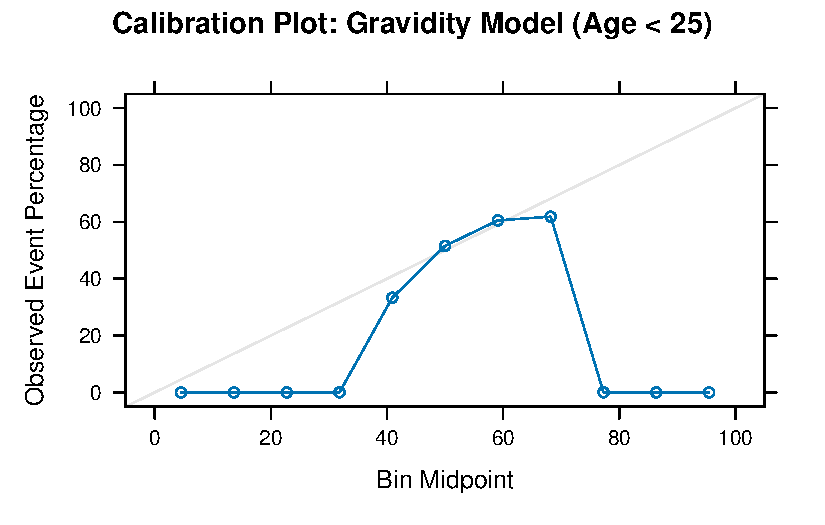
\includegraphics[keepaspectratio]{Supplementary-Material_files/figure-pdf/roc-calibration-2.pdf}}

I see that the ROC curve for my model is close to the diagonal, with an
AUC only slightly above 0.5. This tells me that the model doesn't have
strong discriminative ability for predicting adverse outcomes in women
under 25. Additionally, the calibration plot shows that my predicted
probabilities often stray from the ideal diagonal---especially in the
mid-range---indicating that my model's risk estimates don't consistently
match the observed rates. Overall, while gravidity is statistically
significant, my model as a whole isn't very effective at distinguishing
between those who experience adverse outcomes and those who don't, and
its probability estimates need improvement.

During 5‑fold cross‑validation, the elastic‐net model achieved the
highest mean AUC (0.55±0.01), followed by random forest (0.52±0.01) and
XGBoost (0.50±0.01).

\newpage{}

\section{Discussion}\label{discussion}

\newpage{}

\section{References}\label{references}




\end{document}
